\documentclass[a4paper,12pt]{article}

% Setting up the geometry for the document
\usepackage[margin=1in]{geometry}

% Including essential packages for mathematical typesetting and tables
\usepackage{amsmath, amssymb}
\usepackage{booktabs}
\usepackage{array}
\usepackage{graphicx} % For including images
\usepackage{caption} % For better caption control
\usepackage{subcaption} % For subfigures
\usepackage{siunitx} % For formatting numbers and units
\usepackage{enumitem} % For better enumeration
\usepackage{hyperref} % For hyperlinks
\usepackage{xcolor} % For colored text
\usepackage{fancyhdr} % For custom headers and footers
\usepackage{float} % For better control of float placement

% Setting up the font as requested
\usepackage{mathpazo} % Palatino font with math support

% Ensuring proper spacing and formatting
\usepackage{parskip}
\setlength{\parindent}{0pt}
\setlength{\parskip}{1em}

% Setting up the footer with name
\pagestyle{fancy}
\fancyhf{} % Clear default headers/footers
\fancyfoot[R]{Mohammad Hafizur Rahman Sakib}
\renewcommand{\headrulewidth}{0pt} % No header rule
\renewcommand{\footrulewidth}{0.4pt} % Thin footer rule

\begin{document}

% Title and Introduction
\section*{Introduction}
This lab report, titled \textbf{Neural Network Architectures for Structured and Image Data}, evaluates neural network models on the Pima Indians Diabetes Dataset and the Cassava Plant Disease Dataset. For the diabetes dataset, a Regularized model with dropout and batch normalization is implemented, trained with Adam and SGD optimizers, and uses early stopping to mitigate overfitting. For the Cassava dataset, two convolutional neural network (CNN) models are developed: a custom CNN and a pretrained ResNet50 model, both utilizing data augmentation and early stopping. The report details dataset preprocessing, model architectures, training processes, and performance analysis through accuracy/loss curves and overfitting assessments, highlighting the impact of regularization and data augmentation.

% Section 1: Details of the Datasets
\section*{Details of the Datasets}

\subsection*{Pima Indians Diabetes Dataset}
The Pima Indians Diabetes Dataset, sourced from the UCI Machine Learning Repository, contains 768 instances with 8 feature attributes and 1 binary target variable (Outcome: 1 for diabetes, 0 for no diabetes). Features include:
\begin{itemize}
    \item Pregnancies: Number of times pregnant.
    \item Glucose: Plasma glucose concentration (mg/dL).
    \item BloodPressure: Diastolic blood pressure (mm Hg).
    \item SkinThickness: Triceps skin fold thickness (mm).
    \item Insulin: 2-hour serum insulin (mu U/ml).
    \item BMI: Body mass index (weight in kg/(height in m)$^2$).
    \item DiabetesPedigreeFunction: Genetic predisposition to diabetes.
    \item Age: Age of the patient (years).
\end{itemize}
Missing values (zeros in Glucose, BloodPressure, SkinThickness, Insulin, BMI) are replaced with column means, and features are normalized using StandardScaler.

\section*{Neural Network Model for Diabetes Dataset}
The Regularized model is implemented using TensorFlow/Keras in Google Colab, trained with Adam and SGD optimizers, and uses early stopping (patience=10, monitoring validation loss).

\subsection*{Regularized Model with Dropout and Normalization}
The Regularized model incorporates dropout (20\% rate) and batch normalization to enhance generalization and training stability.

\textbf{Pseudocode:}
\begin{verbatim}
# Preprocess data
Load dataset
Replace zeros with mean in [Glucose, BloodPressure, SkinThickness, Insulin, BMI]
Set features X (all except Outcome), target y (Outcome)
Split data: 80% train, 20% test
Normalize features with StandardScaler

# Define early stopping
Monitor validation loss, patience 10 epochs, restore best weights

# Define model
Sequential model:
    Layer 1: 8 neurons, ReLU, input 8 features
    BatchNormalization
    Dropout (0.2)
    Layer 2: 4 neurons, ReLU
    BatchNormalization
    Dropout (0.2)
    Output: 1 neuron, sigmoid

# Train with Adam
Compile: Adam optimizer, binary crossentropy, accuracy
Train: 100 epochs, batch 32, early stopping
Store history (Adam)

# Train with SGD
Compile: SGD optimizer, binary crossentropy, accuracy
Train: 100 epochs, batch 32, early stopping
Store history (SGD)
\end{verbatim}

\subsection*{Regularized Model Performance}
The Regularized model benefits from dropout to reduce overfitting and batch normalization for stable training. Adam converges faster, while SGD offers steady improvement.

\begin{figure}[H]
    \centering
    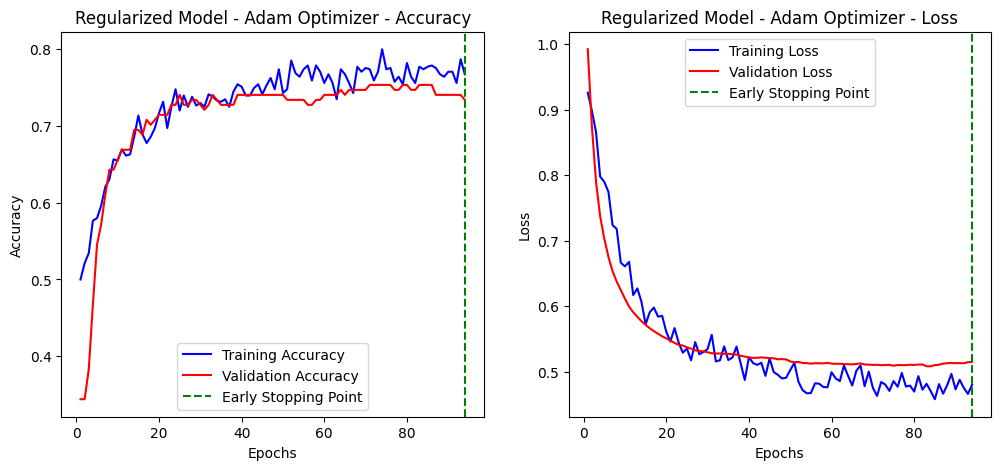
\includegraphics[width=0.8\textwidth]{assets/diabetes/adam_diabetes_loss.png}
    \caption{Performance of Regularized Model (Adam and SGD Optimizers) - Accuracy}
\end{figure}

\begin{figure}[H]
    \centering
    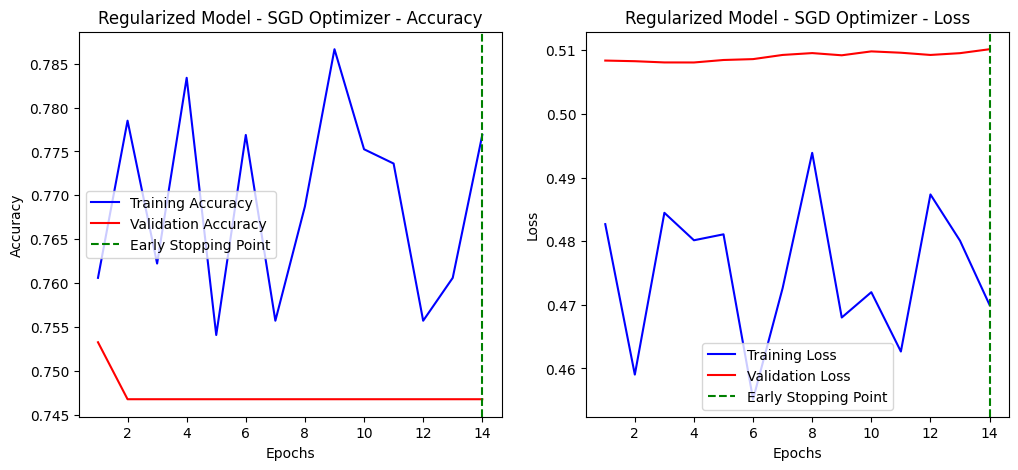
\includegraphics[width=0.8\textwidth]{assets/diabetes/sgd_diabetes_loss.png}
    \caption{Performance of Regularized Model (Adam and SGD Optimizers) - Loss}
\end{figure}



\subsection*{Cassava Plant Disease Dataset}
The Cassava Plant Disease Dataset contains images of cassava leaves, labeled into five classes: Cassava Bacterial Blight (CBB), Cassava Brown Streak Disease (CBSD), Cassava Green Mottle (CGM), Cassava Mosaic Disease (CMD), and Healthy. The dataset includes:
\begin{itemize}
    \item \textbf{train\_images}: Folder with images resized to 224x224 pixels (RGB).
    \item \textbf{label\_num\_to\_disease\_map.json}: JSON file mapping labels (0–4) to disease names.
    \item \textbf{train.csv}: CSV file mapping image filenames to labels.
\end{itemize}
The dataset has ~21,000 images, with ~20\% per class, split into 80\% training and 20\% testing. Images are normalized to [0,1], and data augmentation is applied.

\subsubsection*{Sample Images}
Below are sample images, including a primary image (`test.png`) and representatives of each class:

\begin{figure}[H]
    \centering
    \begin{subfigure}{0.45\textwidth}
        \centering
        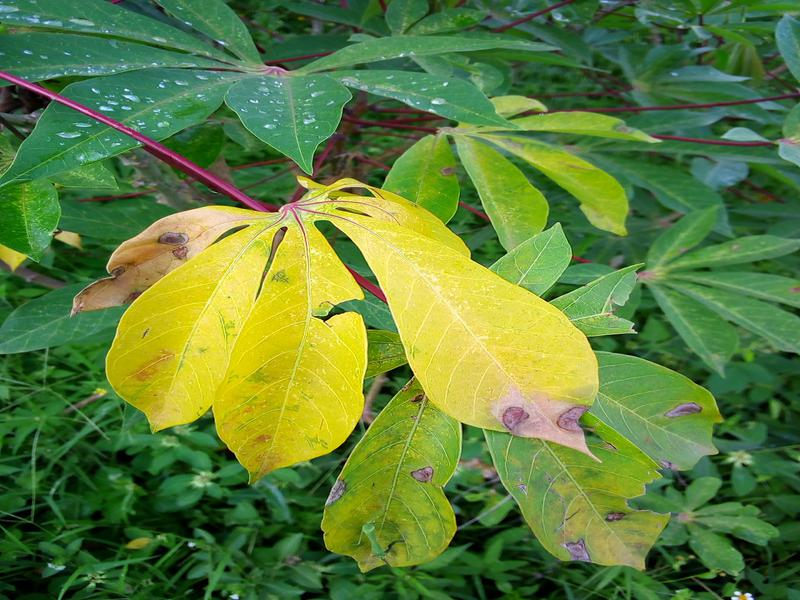
\includegraphics[width=\textwidth]{./assets/class_images/class_0.jpg}
        \caption{Cassava Bacterial Blight (CBB)}
    \end{subfigure}
    \hfill
    \begin{subfigure}{0.45\textwidth}
        \centering
        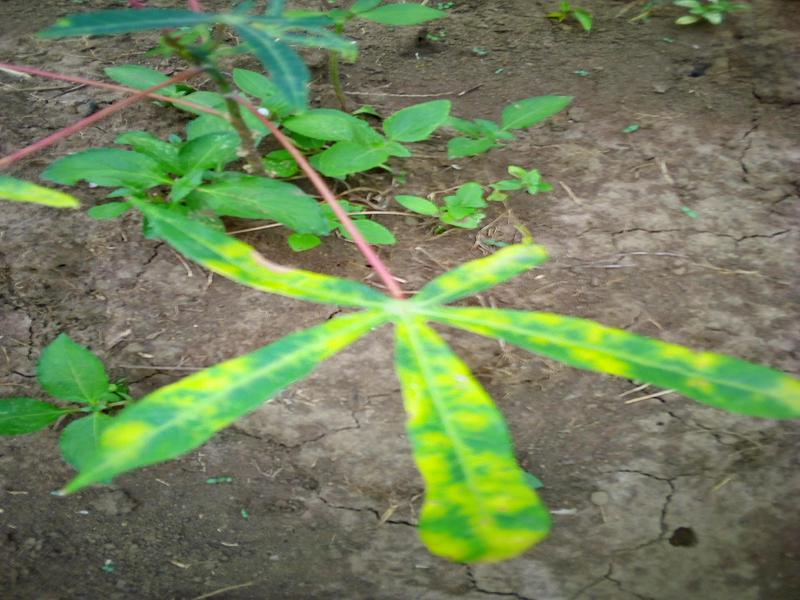
\includegraphics[width=\textwidth]{./assets/class_images/class_1.jpg}
        \caption{Cassava Brown Streak Disease (CBSD)}
    \end{subfigure}
    
    \vspace{0.5cm}
    
    \begin{subfigure}{0.45\textwidth}
        \centering
        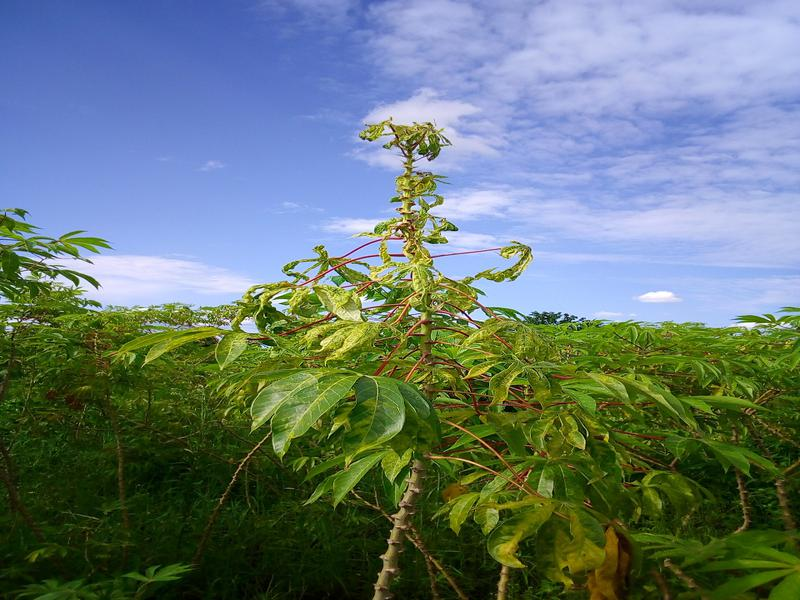
\includegraphics[width=\textwidth]{./assets/class_images/class_2.jpg}
        \caption{Cassava Green Mottle (CGM)}
    \end{subfigure}
    \hfill
    \begin{subfigure}{0.45\textwidth}
        \centering
        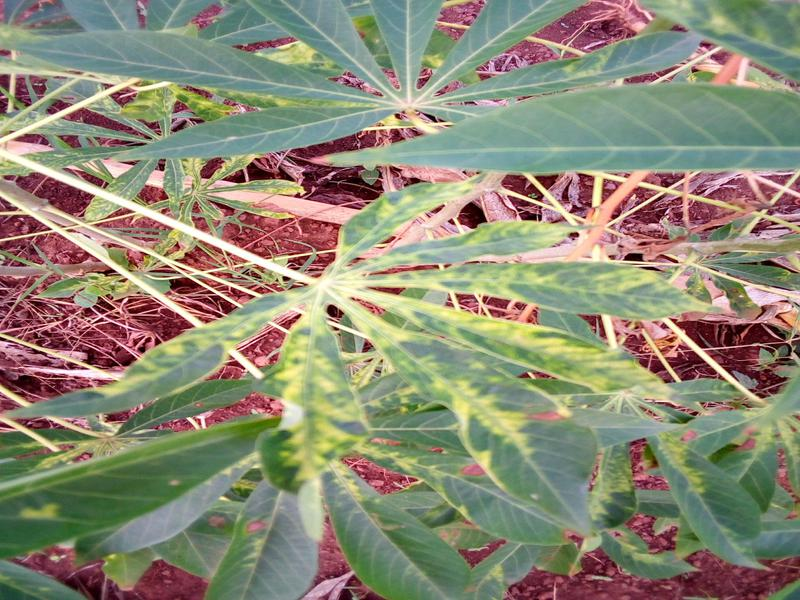
\includegraphics[width=\textwidth]{./assets/class_images/class_3.jpg}
        \caption{Cassava Mosaic Disease (CMD)}
    \end{subfigure}
    
    \vspace{0.5cm}
    
    \centering
    \begin{subfigure}{0.45\textwidth}
        \centering
        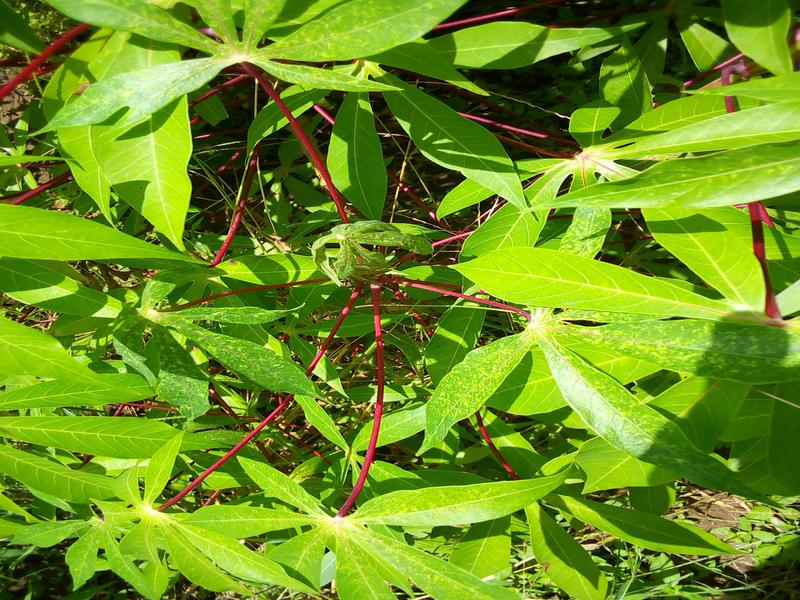
\includegraphics[width=\textwidth]{./assets/class_images/class_4.jpg}
        \caption{Healthy}
    \end{subfigure}
    \caption{Sample images from the Cassava Plant Disease Dataset}
\end{figure}

% Section 2: Target and Feature Selection
\section*{Target and Feature Selection}
\subsection*{Cassava Plant Disease Dataset}
The target is a categorical label (0: CBB, 1: CBSD, 2: CGM, 3: CMD, 4: Healthy). Features are pixel intensities from 224x224x3 images, normalized with data augmentation.


% Section 4: Neural Network Models for Cassava Dataset
\section*{Neural Network Models for Cassava Dataset}
Two CNN models are implemented: a custom CNN and a pretrained ResNet50 model, both using data augmentation and early stopping (patience=10, monitoring validation loss) to address overfitting/underfitting. Models are trained with Adam optimizer in Google Colab.

\subsection*{Data Augmentation}
Data augmentation enhances model robustness with:
\begin{itemize}
    \item Rotation: Up to 20 degrees.
    \item Horizontal Flip: Randomly flip images.
    \item Zoom: Up to 20\% zoom range.
    \item Shear: Up to 20\% shear range.
\end{itemize}
Augmented outputs (e.g., rotated CBB, flipped CMD) increase dataset diversity:

\begin{figure}[H]
    \centering
    \includegraphics[width=0.8\textwidth]{example-image}
    \caption{Examples of Augmented Cassava Images (Rotation, Flip, Zoom, Shear)}
\end{figure}

\subsection*{Custom CNN Model}
\textbf{Pseudocode:}
\begin{verbatim}
# Preprocess data
Load train.csv, train_images, label_num_to_disease_map.json
Normalize pixel values to [0,1]
Apply data augmentation (rotation, flip, zoom)
Split data: 80% train, 20% test

# Define early stopping
Monitor validation loss, patience 10 epochs, restore best weights

# Define model
Sequential model:
    Conv2D: 32 filters, 3x3, ReLU, input 224x224x3
    MaxPooling2D: 2x2
    Conv2D: 64 filters, 3x3, ReLU
    MaxPooling2D: 2x2
    Conv2D: 128 filters, 3x3, ReLU
    MaxPooling2D: 2x2
    Flatten
    Dense: 128 neurons, ReLU
    Dropout (0.5)
    Dense: 5 neurons, softmax

# Train with Adam
Compile: Adam optimizer, categorical crossentropy, accuracy
Train: 50 epochs, batch 32, early stopping
Store history
\end{verbatim}

\subsection*{Custom CNN Performance}
\begin{figure}[H]
    \centering
    \includegraphics[width=0.8\textwidth]{example-image}
    \caption{Performance of Custom CNN Model (Adam Optimizer) - Accuracy and Loss}
\end{figure}

\subsection*{Pretrained ResNet50 Model}
The ResNet50 model uses pretrained ImageNet weights with a frozen convolutional base and a custom classifier.

\textbf{Pseudocode:}
\begin{verbatim}
# Preprocess data (same as above)

# Define early stopping
Monitor validation loss, patience 10 epochs, restore best weights

# Define model
Load ResNet50 (pretrained, exclude top)
Freeze convolutional layers
Add layers:
    GlobalAveragePooling2D
    Dense: 128 neurons, ReLU
    Dropout (0.5)
    Dense: 5 neurons, softmax

# Train with Adam
Compile: Adam optimizer, categorical crossentropy, accuracy
Train: 50 epochs, batch 32, early stopping
Store history
\end{verbatim}

\subsection*{Pretrained ResNet50 Performance}
\begin{figure}[H]
    \centering
    \includegraphics[width=0.8\textwidth]{example-image}
    \caption{Performance of Pretrained ResNet50 Model (Adam Optimizer) - Accuracy and Loss}
\end{figure}

% Section 5: Early Stopping
\section*{Early Stopping}
Early stopping (patience=10, monitoring validation loss) is applied to all models to prevent overfitting and address underfitting by restoring best weights. This is critical for the CNN models due to their high capacity.

% Section 6: Optimizers
\section*{Optimizers}
\begin{itemize}
    \item \textbf{Adam}: Used for all models, offering fast convergence via adaptive learning rates.
    \item \textbf{SGD}: Used for the diabetes model, providing stable but slower convergence.
\end{itemize}

% Section 7: Loss Graphs
\section*{Loss Graphs}
Loss curves compare model performance:

\begin{figure}[H]
    \centering
    \includegraphics[width=0.8\textwidth]{example-image}
    \caption{Loss Curves for Regularized Diabetes Model (Adam and SGD Optimizers)}
\end{figure}

\begin{figure}[H]
    \centering
    \includegraphics[width=0.8\textwidth]{example-image}
    \caption{Loss Curves for Cassava Models (Custom CNN and ResNet50, Adam Optimizer)}
\end{figure}

% Section 8: Overfitting Analysis
\section*{Overfitting Analysis}
The diabetes model is trained without early stopping for 500 epochs to induce overfitting, showing divergent validation loss. For Cassava models, data augmentation and dropout mitigate overfitting, with early stopping ensuring optimal performance.

\begin{figure}[H]
    \centering
    \includegraphics[width=0.8\textwidth]{example-image}
    \caption{Overfitting Analysis for Regularized Diabetes Model}
\end{figure}

\begin{figure}[H]
    \centering
    \includegraphics[width=0.8\textwidth]{example-image}
    \caption{Overfitting Analysis for Cassava Crop Diseases Classification Custom Models}
\end{figure}

\begin{figure}[H]
    \centering
    \includegraphics[width=0.8\textwidth]{example-image}
    \caption{Overfitting Analysis for Cassava Crop Diseases Classification Pretrained CNN Model}
\end{figure}

% Section 9: Findings
\section*{Findings}
\begin{itemize}
    \item \textbf{Diabetes Dataset}:
    \begin{itemize}
        \item The Regularized model with dropout and batch normalization improved generalization.
        \item SGD provided stable performance, potentially outperforming Adam in F1-score.
        \item Early stopping was critical to prevent overfitting.
    \end{itemize}
    \item \textbf{Cassava Dataset}:
    \begin{itemize}
        \item Data augmentation (rotation, flip, zoom) enhanced robustness, as seen in augmented images.
        \item ResNet50 outperformed the custom CNN due to pretrained features.
        \item Early stopping and dropout effectively controlled overfitting.
    \end{itemize}
    \item \textbf{Recommendations}: Use the Regularized model with SGD for diabetes prediction and ResNet50 with data augmentation for cassava disease classification.
\end{itemize}

\end{document}